% Copyright (c) 2014,2015 Jeremie DECOCK (http://www.jdhp.org)

% This document is provided under the terms of the "Creative Commons BY-SA" license.
% For more details, read the "COPYING/legalcode.html" enclosed file or
% the "http://creativecommons.org/licenses/by-sa/4.0/legalcode" web page.

\documentclass{article}

\usepackage[utf8]{inputenc}
\usepackage[T1]{fontenc}

% English environment
%\usepackage[english]{babel}

% French environment
\usepackage[french]{babel}

% French + English environment
%\usepackage[francais,english]{babel}

%%%%%%%%%%%%%%%%%%%%%%%%%%%%%%%%%%%%%%%%%%%%%%%%%%%%%%%%%%%%%%%%%%%%%%%%%%%%%%%%

% Clickable Table of Contents
% http://tex.stackexchange.com/questions/73862/how-can-i-make-a-clickable-table-of-contents
\usepackage{hyperref}
\hypersetup{
	pdftoolbar=true,                                          % show Acrobat’s toolbar ?
	pdfmenubar=true,                                          % show Acrobat’s menu ?
	pdffitwindow=true,                                        % page fit to window when opened
	pdfnewwindow=true,                                        % links in new window
	colorlinks=true,                                          % false: boxed links; true: colored links
	linkcolor=black,                                          % color of internal links
	citecolor=black,                                          % color of links to bibliography
	filecolor=black,                                          % color of file links
	urlcolor=black                                            % color of external links
}

\usepackage{algorithm}
\usepackage{algorithmic}
\usepackage{amsmath}
\usepackage{amssymb}
%\usepackage{bm}    % bold math
\usepackage{color}  % change text color
\usepackage{xcolor} % required for listings package...
\usepackage{epsfig}
\usepackage{eurosym}
\usepackage{flushend}
\usepackage{graphicx}
\usepackage{ifthen}
\usepackage{multirow}
%\usepackage{natbib} % For bibliography, often used nowadays
\usepackage{subfigure}
\usepackage{url}

%% Inserting a pdf file in the document
%% See: http://stackoverflow.com/questions/2739159/inserting-a-pdf-file-in-latex 
%\usepackage{pdfpages}
%\usepackage{epsfig}
%\usepackage{geometry}
%\usepackage{pdflscape}

%%%%%%%%%%%%%%%%%%%%%%%%%%%%%%%%%%%%%%%%%%%%%%%%%%%%%%%%%%%%%%%%%%%%%%%%%%%%%%%%

%\usepackage[font=sf, labelfont={sf,bf}, margin=1cm]{caption}
%\usepackage[font=rm, margin=1cm]{caption}

% HeVeA %%%%%%%%%%%%%%%%%%%%%%%%%%%%%%%%%%%%%%%%%%%%%%%%%%%%%%%%%%%%%%%%%%%%%%%

\usepackage{hevea}
\newstyle{body}{margin-left: auto; margin-right: auto; padding: .5em 1.5em; max-width: 50em; text-align: justify; font-family: sans-serif;}
\newstyle{div.lstlisting}{font-size: 130\%; margin-left: auto; margin-right: auto; width: 35em;}

\newif\ifpdf                   
\ifx\pdfoutput\undefined
\pdffalse
\else
\pdfoutput=1
\pdftrue
\fi

% TikZ %%%%%%%%%%%%%%%%%%%%%%%%%%%%%%%%%%%%%%%%%%%%%%%%%%%%%%%%%%%%%%%%%%%%%%%%

%\usepackage{tikz}
%\input{setup_package_tikz.tex}

% Listings package settings %%%%%%%%%%%%%%%%%%%%%%%%%%%%%%%%%%%%%%%%%%%%%%%%%%%%

\usepackage{listings}

% Listings package settings %%%%%%%%%%%%%%%%%%%%%%%%%%%%%%%%%%%%%%%%%%%%%%%%%%%%

% See http://en.wikibooks.org/wiki/LaTeX/Source_Code_Listings

% By default, listings does not support multi-byte encoding for source code. The extendedchar option only works for 8-bits encodings such as latin1.
% To handle UTF-8, you should tell listings how to interpret the special characters by defining them like so
\lstset{literate=
    {á}{{\'a}}1 {é}{{\'e}}1 {í}{{\'i}}1 {ó}{{\'o}}1 {ú}{{\'u}}1
    {Á}{{\'A}}1 {É}{{\'E}}1 {Í}{{\'I}}1 {Ó}{{\'O}}1 {Ú}{{\'U}}1
    {à}{{\`a}}1 {è}{{\'e}}1 {ì}{{\`i}}1 {ò}{{\`o}}1 {ù}{{\`u}}1
    {À}{{\`A}}1 {È}{{\'E}}1 {Ì}{{\`I}}1 {Ò}{{\`O}}1 {Ù}{{\`U}}1
    {ä}{{\"a}}1 {ë}{{\"e}}1 {ï}{{\"i}}1 {ö}{{\"o}}1 {ü}{{\"u}}1
    {Ä}{{\"A}}1 {Ë}{{\"E}}1 {Ï}{{\"I}}1 {Ö}{{\"O}}1 {Ü}{{\"U}}1
    {â}{{\^a}}1 {ê}{{\^e}}1 {î}{{\^i}}1 {ô}{{\^o}}1 {û}{{\^u}}1
    {Â}{{\^A}}1 {Ê}{{\^E}}1 {Î}{{\^I}}1 {Ô}{{\^O}}1 {Û}{{\^U}}1
    {œ}{{\oe}}1 {Œ}{{\OE}}1 {æ}{{\ae}}1 {Æ}{{\AE}}1 {ß}{{\ss}}1
    {ç}{{\c c}}1 {Ç}{{\c C}}1 {ø}{{\o}}1 {å}{{\r a}}1 {Å}{{\r A}}1
    {€}{{\EUR}}1 {£}{{\pounds}}1
}

\usepackage{color}

\definecolor{mygreen}{rgb}{0,0.6,0}
\definecolor{mygray}{rgb}{0.5,0.5,0.5}
\definecolor{mymauve}{rgb}{0.58,0,0.82}

\lstset{ %
  backgroundcolor=\color{white},   % choose the background color; you must add \usepackage{color} or \usepackage{xcolor}
  basicstyle=\footnotesize,        % the size of the fonts that are used for the code
  breakatwhitespace=false,         % sets if automatic breaks should only happen at whitespace
  breaklines=true,                 % sets automatic line breaking
  captionpos=b,                    % sets the caption-position to bottom
  commentstyle=\color{mygreen},    % comment style
  deletekeywords={...},            % if you want to delete keywords from the given language
  escapeinside={\%*}{*)},          % if you want to add LaTeX within your code
  extendedchars=true,              % lets you use non-ASCII characters; for 8-bits encodings only, does not work with UTF-8
  frame=L,                    % adds a frame around the code
  keepspaces=true,                 % keeps spaces in text, useful for keeping indentation of code (possibly needs columns=flexible)
  keywordstyle=\color{blue},       % keyword style
  %language=Octave,                % the language of the code
  morekeywords={*,...},            % if you want to add more keywords to the set
  numbers=left,                    % where to put the line-numbers; possible values are (none, left, right)
  numbersep=10pt,                  % how far the line-numbers are from the code
  numberstyle=\tiny\color{mygray}, % the style that is used for the line-numbers
  rulecolor=\color{black},         % if not set, the frame-color may be changed on line-breaks within not-black text (e.g. comments (green here))
  showspaces=false,                % show spaces everywhere adding particular underscores; it overrides 'showstringspaces'
  showstringspaces=false,          % underline spaces within strings only
  showtabs=false,                  % show tabs within strings adding particular underscores
  stepnumber=1,                    % the step between two line-numbers. If it's 1, each line will be numbered
  stringstyle=\color{mymauve},     % string literal style
  tabsize=2,                       % sets default tabsize to 2 spaces
  title=\lstname                   % show the filename of files included with \lstinputlisting; also try caption instead of title
}

\lstdefinestyle{customc}{
  belowcaptionskip=1\baselineskip,
  breaklines=true,
  frame=L,
  xleftmargin=\parindent,
  language=C,
  showstringspaces=false,
  basicstyle=\footnotesize\ttfamily,
  keywordstyle=\bfseries\color{green!40!black},
  commentstyle=\itshape\color{purple!40!black},
  identifierstyle=\color{blue},
  stringstyle=\color{orange},
}

\lstdefinestyle{customasm}{
  belowcaptionskip=1\baselineskip,
  frame=L,
  xleftmargin=\parindent,
  language=[x86masm]Assembler,
  basicstyle=\footnotesize\ttfamily,
  commentstyle=\itshape\color{purple!40!black},
}

\lstset{escapechar=@,style=customc}



%% COMMANDS AND DEFS %%%%%%%%%%%%%%%%%%%%%%%%%%%%%%%%%%%%%%%%%%%%%%%%%%%%%%%%%%%

% Pour désactiver temporairement les images (compile beaucoup plus vite)
%\renewcommand{\includegraphics}[2][]{\null}

%%% Math symbols

%\renewcommand{\vec}[1]{\ensuremath{\boldsymbol{#1}}} % bold vectors
\newcommand{\vs}[1]{\boldsymbol{#1}} % vector symbol (\boldsymbol, \textbf or \vec)
\newcommand{\ms}[1]{\boldsymbol{#1}} % matrix symbol (\boldsymbol, \textbf)

\newcommand{\x}{\vs{x}}
\newcommand{\xstar}{\vs{x^*}}
\newcommand{\w}{\vs{\omega}}
\newcommand{\objfunc}{f}

\def\bbbr{{\rm I\!R}} % reelle Zahlen

\newcommand{\E}{\mathbb{E}}
\newcommand{\N}{\mathbb{N}}
\newcommand{\Z}{\mathbb{Z}}
\newcommand{\Q}{\mathbb{Q}}
\newcommand{\R}{{\bbbr}{}}
\newcommand{\C}{\mathbb{C}}
\newcommand{\K}{\mathbb{K}}

\newcommand{\mb}[1]{\mathbb{#1}}
\newcommand{\mc}[1]{\mathcal{#1}}

\def\CQFD{\fbox\\}

%%% General commands

\newenvironment{jmatrix}{\renewcommand\arraystretch{1.5} \begin{pmatrix}}{\end{pmatrix}}
%\renewcommand{\arraystretch}{1.5}

\newcommand{\cred}[1]{\textcolor{red}{#1}}
\newcommand{\ech}[1]{\textcolor{gray}{#1}}
\newcommand{\imp}[1]{{\em {#1}}}
\newcommand{\voc}[1]{{\em {#1}}}
\newcommand{\todo}[1][\dots]{\textbf{[TODO : #1]}}  % todo mark

\newcommand{\dontforget}[1]{\textcolor{red}{#1}}

\newcommand{\HRule}{\rule{\linewidth}{0.5mm}}

%%% Debug: Display the current table counter (cf. http://www.iam.ubc.ca/old_pages/newbury/tex/numbering.html)

\newcommand{\tablecounterdebug}{\textbf{Table~counter:~\thetable}\\}
\newcommand{\equationcounterdebug}{\textbf{Equation~counter:~\theequation}\\}
\newcommand{\figurecounterdebug}{\textbf{Figure~counter:~\thefigure}\\}
\newcommand{\algorithmcounterdebug}{\textbf{Algorithm~counter:~\thealgorithm}\\}



\sloppy

%%%%%%%%%%%%%%%%%%%%%%%%%%%%%%%%%%%%%%%%%%%%%%%%%%%%%%%%%%%%%%%%%%%%%%%%%%%%%%%

\title{Émuler le Raspberry Pi sous Debian avec Qemu}

\author{Jérémie \textsc{Decock} \\ \url{http://www.jdhp.org}}

%\institute{ \textsuperscript{1}TAO, INRIA-CNRS-LRI, Univ. Paris-Sud, 91190 Gif-sur-Yvette, France}
\date{Janvier 2015}

\hypersetup{
	pdftitle={Émuler le Raspberry Pi sous Debian avec Qemu},     % title
	pdfauthor={Jérémie DECOCK},      % author
	pdfsubject={Émuler le Raspberry Pi avec Qemu}, % subject of the document
	pdfkeywords={émulateur, qemu, raspberry pi, debian}         % list of keywords
}

%%%%%%%%%%%%%%%%%%%%%%%%%%%%%%%%%%%%%%%%%%%%%%%%%%%%%%%%%%%%%%%%%%%%%%%%%%%%%%%

\begin{document}

\maketitle

\tableofcontents

% Introduction %%%%%%%%%%%%%%%%%%%%%%%%%%%%%%%%%%%%%%%%%%%%%%%%%%%%%%%%%%%%%%%%

\section*{Introduction}\label{sec:intro}

% Qu'est-ce que Qemu ?
Qemu est un logiciel libre de virtualisation, capable de simuler un grand
nombre d'architectures matérielles.
Il est notamment capable de simuler le processeur ARM 1176JZFS contenu dans
le SoC\footnote{Système sur une puce, un système complet embarqué sur un seul
circuit intégré, pouvant comprendre un ou plusieurs processeurs, de la mémoire,
des contrôleurs et des périphériques.} Broadcom BCM2835 du Raspberry Pi.
%\footnote{Les Raspberry Pi modèle A, A+, B et B+ utilisent le même SoC Broadcom BCM2835.}.
% Intérêt/usage
Avec Qemu, il est ainsi possible de manipuler un ou plusieurs Raspberry Pi
virtuels dans un ordinateur hôte.
Cette virtualisation du Raspberry Pi est très utile pour configurer et tester
rapidement des environnements logiciels.
Elle permet entre autre de simplifier la création de sauvegardes lors de la
mise au point de ces environnements.
%de cette plate-forme
Elle permet également d'épargner les longs transferts de données avec les cartes SD
%utilisées pour les stocker.
qui sont utilisées comme support de stockage principale du Raspberry Pi.
%Elle permet entre autre d'épargner les longs transferts de données avec la
%carte SD contenant l'environnement logiciel de cette plate-forme
%et simplifie la création de sauvegardes lors de la mise au point de l'environnement logiciel.

\begin{figure}
    \centering
    \ifpdf
    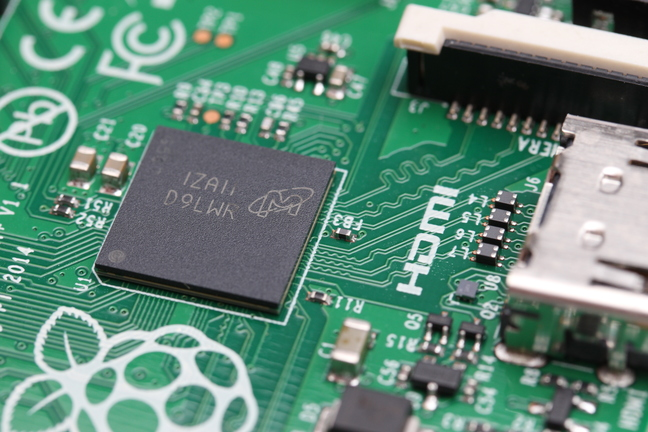
\includegraphics[width=.70\linewidth]{fig/bcm2835.jpeg}
    \else
    \imgsrc{fig/bcm2835.jpeg}
    \fi
    \caption{\label{fig:bcm2835}Le SoC Broadcom BCM2835 d'un Raspberry Pi A+.} %\footnote{Ici fabriqué par l'entreprise Micron.}
\end{figure}


Dans ce tutoriel, nous verrons comment émuler un Raspberry Pi avec Qemu sur un
système hôte Gnu/Linux Debian Jessie.
L'émulation sur Mac OS X et Microsoft Windows est également possible mais n'est
pas abordée ici.
%\cred{pour ces os, se référer \cite{xecdesign1}.}


% Section 1 %%%%%%%%%%%%%%%%%%%%%%%%%%%%%%%%%%%%%%%%%%%%%%%%%%%%%%%%%%%%%%%%%%%

\section{Installer Qemu}\label{sec:intall-qemu}

Commençons par installer Qemu sur le système hôte.  Pour Debian Jessie, il
suffit d'installer le paquet {\em qemu-system-arm}~:
\begin{verbatim}
# apt-get install qemu-system-arm
\end{verbatim}
% # apt-get install qemu qemu-system-arm qemu-utils

%Fedora: qemu-system-arm et qemu-user.

Si vous utilisez un autre système d'exploitation que Debian Jessie ou que vous
compilez vous-même Qemu, vérifiez que le processeur ARM1176 du Raspberry Pi est
bien supporté avec la commande
\begin{verbatim}
$ qemu-arm -cpu help
\end{verbatim}
Cette commande liste les processeurs ARM pris en charge.
Assurez-vous que l'arm1176 y figure.


% Section 1 %%%%%%%%%%%%%%%%%%%%%%%%%%%%%%%%%%%%%%%%%%%%%%%%%%%%%%%%%%%%%%%%%%%

%\section{Récupérer une distribution Gnu/Linux et un noyau Linux pour le Raspberry Pi}\label{sec:get-distro-and-kernel}
\section{Récupérer un système et un noyau pour le Raspberry Pi}\label{sec:get-distro-and-kernel}

L'étape suivante consiste à télécharger l'image du système à émuler.
Les images officiellement supportées par la fondation Raspberry Pi
sont accessibles sur la page
\url{http://www.raspberrypi.org/downloads/}
et de nombreuses autres sont disponibles sur le web.
%
% j'utilise vs nous utilisons
Dans ce tutoriel, nous utilisons le système {\em Raspbian 2014-12-24} téléchargeable sur
\url{http://downloads.raspberrypi.org/raspbian/images/raspbian-2014-12-25/2014-12-24-wheezy-raspbian.zip}~%;
(ce fichier doit être décompressé pour obtenir l'image système \og{}2014-12-24-wheezy-raspbian.img\fg{}).
%une fois décompressé, le fichier 2014-12-24-wheezy-raspbian.img
%contient l'image du système.

Nous allons également avoir besoin d'un noyau Linux particulier, compilé pour être utilisable avec Qemu.
La page
\href{https://web.archive.org/web/20150214035104/http://xecdesign.com/compiling-a-kernel/}{http://xecdesign.com/compiling-a-kernel/}
explique comment compiler un tel noyau.
Vous pouvez également télécharger un noyau tout prêt à l'adresse suivante~:
\href{https://web.archive.org/web/20150419093434/http://www.xecdesign.com/downloads/linux-qemu/kernel-qemu}{http://xecdesign.com/downloads/linux-qemu/kernel-qemu}.

%On suppose ...img et kernel-qemu sont dans le répertoire courant du terminal.

% Section 2 %%%%%%%%%%%%%%%%%%%%%%%%%%%%%%%%%%%%%%%%%%%%%%%%%%%%%%%%%%%%%%%%%%%

\section{Préparation de l'image du système}\label{sec:setup-image}

Dans le cas de Raspbian, l'image système n'est pas directement utilisable par
Qemu et nécessite quelques modifications.
% (c'est probablement le cas avec d'autres distributions).
% aménagements
Les images système du Raspberry Pi contiennent un disque complet avec un MBR et
plusieurs partitions (deux dans le cas de Raspbian) ce qui complique un peu
leur manipulation\footnote{Voir par exemple le commentaire de Gordon Hollingworth sur \url{http://www.raspberrypi.org/forums/viewtopic.php?f=29&t=48811&p=380844&hilit=kpartx\#p380844}.}.
%\cred{et non pas une simple partition, ce qui complique légèrement leur accès.
Néanmoins, plusieurs techniques existent pour modifier ce type d'images système
\footnote{
    Certains tutoriels utilisent par exemple la commande {\em mount} avec l'option
    \og{}-o loop,offset=XXX\fg{}, où XXX est l'index du premier bit de la partition
    à monter
    %dans l'image système
    (récupérable avec les commandes {\em fdisk} et {\em file}).
    D'autres effectuent les modifications via une instance minimale du système
    émulé dans Qemu, en désignant un shell comme processus initial, via l'option
    \og{}init=/bin/bash\fg{} du noyau (ce que de nombreux systèmes appellent le
    \og{}mode de maintenance\fg{}).
    Mais je trouve plus propre et plus souple d'effectuer les modifications
    depuis le système hôte et de générer automatiquement les périphériques
    correspondant aux partitions de l'image système via la commande {\em
    kpartx}.
    % Plusieurs techniques existent pour modifier l'image système.
    % Certains tutoriels expliquent comment effectuer ces modifications via une
    % instance minimale du système émulé dans Qemu, en désignant un shell comme
    % processus initial, via l'option \og{}init=/bin/bash\fg{} au noyau (ce que de
    % nombreux systèmes appellent le \og{}mode maintenance\fg{}).
    % D'autres préconisent d'utiliser la commande {\em mount} avec l'option \og{}-o
    % loop,offset=XXX\fg{}, où XXX est l'index du premier bit de la partition à
    % monter dans l'image système (préalablement récupéré avec les commandes {\em fdisk} ou {\em
    % file}).

    % Pour modifier une image système, nous avons besoin de monter les partitions qu'elle contient.
    % Comme les images systèmes utilisées pour le Raspberry Pi contiennent plusieurs
    % partitions, il n'est pas possible de les monter directement avec la commande {\em mount}.
} et nous utiliserons ici la commande {\em kpartx} pour effectuer ces modifications. % depuis le système hôte.
%Kpartx doit préalablement être installé sur le système hôte.
%Pour Debian, il suffit d'installer le paquet {\em kpartx}.
Sur Debian, il faut préalablement installer le paquet {\em kpartx}~:

\begin{verbatim}
# apt-get install kpartx
\end{verbatim}

%\cred{Les images système contiennent des }.
%Elles contiennent un MBR et des partitions.

%%% Pour modifier une image système, nous avons besoin de monter les partitions qu'elle contient.
%%% Comme les images systèmes utilisées pour le Raspberry Pi contiennent plusieurs
%%% partitions, il n'est pas possible de les monter directement avec la commande {\em mount}.

Les périphériques correspondant aux partitions peuvent ensuite être générés avec la commande

% http://askubuntu.com/questions/445979/mount-sd-card-image-created-using-dd
\begin{verbatim}
# kpartx -av 2014-12-24-wheezy-raspbian.img
\end{verbatim}

Cette commande crée les périphériques /dev/mapper/loop0p1 et /dev/mapper/loop0p2
correspondant aux deux partitions contenues dans l'image {\em
2014-12-24-wheezy-raspbian.img}.
% pour raspbian... il peut y avoir plus de partitions pour d'autres distrib...
Seule la deuxième partition nous intéresse ici (celle qui contient la {\em racine}
du système) et nous pouvons la monter normalement avec les commandes~:
%Ces partitions peuvent être montées normalement~:
\begin{verbatim}
# mkdir /mnt/loop0p2
# mount /dev/mapper/loop0p2 /mnt/loop0p2
\end{verbatim}

L'arborescence de la Raspbian est alors accessible et modifiable dans le
répertoire \og{}/mnt/loop0p2\fg{}.

La première modification à apporter consiste à désactiver l'utilisation
de la bibliothèque {\em cofi\_rpi}, propre au Raspberry Pi et inutilisable dans
Qemu\footnote{La bibliothèque cofi\_rpi (libcofi\_rpi.so) propose une
    implémentation propre au Raspberry Pi des fonctions {\em memcpy} et {\em
    memset} de la librairie standard. Elle améliore la performance des
    programmes en exploitant l'accélération matérielle du Raspberry Pi (cf.
    \url{http://www.raspberrypi.org/forums/viewtopic.php?f=63&t=9260}).
    %with the intention of gaining greater
    %performance.\url{http://archlinuxarm.org/forum/viewtopic.php?f=31&t=5684}
}.
Pour ce faire, éditez le fichier \og{}/mnt/loop0p2/etc/ld.so.preload\fg{} et
commentez son contenu en mettant un \# au tout début de la ligne suivante~:
\begin{verbatim}
/usr/lib/arm-linux-gnueabihf/libcofi_rpi.so
\end{verbatim}
Sans cette modification, Raspbian plantera au démarrage dans Qemu.

La seconde modification est utile mais pas indispensable.
Elle consiste à corriger une différence de nommage des périphériques de stockage entre
le noyau utilisé pour Qemu et le noyau de Raspbian.
Cette différence est susceptible de générer quelques erreurs.
Pour corriger ce problème, il faut éditer le fichier \og{}/mnt/loop0p2/etc/udev/rules.d/90-qemu.rules\fg{}
avec le contenu suivant~:
\begin{verbatim}
KERNEL=="sda", SYMLINK+="mmcblk0"
KERNEL=="sda?", SYMLINK+="mmcblk0p%n"
KERNEL=="sda2", SYMLINK+="root"
\end{verbatim}

Le noyau utilisé par Qemu voit le disque \og{}/dev/sda\fg{}, alors que le
\og{}vrai\fg{} noyau de la Raspbian voit \og{}/dev/mmcblk0\fg{}.
Notre modification permet de créer des liens symboliques pour être plus
proche du vrai Raspberry Pi.

Une fois ces ajustements opérés, nous pouvons démonter la partition {\em
loop0p2} et supprimer les périphériques précédemment générés~:
\begin{verbatim}
# umount /mnt/loop0p2
# kpartx -d 2014-12-24-wheezy-raspbian.img
\end{verbatim}


% http://www.raspberrypi.org/forums/viewtopic.php?f=29&t=48811&p=380844&hilit=kpartx
% $ sudo losetup /dev/loop0 raspbian.img
% $ sudo kpartx /dev/loop0
% $ sudo mount /dev/mapper/loop0p1 /mnt/part1
% $ sudo mount /dev/mapper/loop0p5 /mnt/part5
% $ sudo mount /dev/mapper/loop0p6 /mnt/part6

% http://fr.docs.kali.org/development-fr/image-raspberry-pi-personaliser
% loopdevice=`losetup -f --show kali-custom-rpi.img`
% device=`kpartx -va $loopdevice| sed -E 's/.*(loop[0-9])p.*/1/g' | head -1`
% device="/dev/mapper/${device}"
% bootp=${device}p1
% rootp=${device}p2
% mkfs.vfat $bootp
% mkfs.ext4 $rootp
% mkdir -p root
% mkdir -p boot
% mount $rootp root
% mount $bootp boot

% http://raspberrypi.stackexchange.com/questions/13137/how-can-i-mount-a-raspberry-pi-linux-distro-image

% http://elinux.org/RPi_Easy_SD_Card_Setup

% http://linuxconfig.org/how-to-mount-rasberry-pi-filesystem-image
% http://www.raspberrypi.org/forums/viewtopic.php?f=63&t=28860


%\begin{verbatim}
%$ qemu-system-arm \
%    -kernel kernel-qemu \
%    -cpu arm1176 \
%    -m 256 \
%    -M versatilepb \
%    -no-reboot \
%    -serial stdio \
%    -append "root=/dev/sda2 panic=1 rootfstype=ext4 rw init=/bin/bash" \
%    -hda 2014-12-24-wheezy-raspbian.img
%\end{verbatim}

% Section 3 %%%%%%%%%%%%%%%%%%%%%%%%%%%%%%%%%%%%%%%%%%%%%%%%%%%%%%%%%%%%%%%%%%%

\section{Premier démarrage}\label{sec:first-boot}

Maintenant que l'image du système est prête, nous allons pouvoir démarrer l'émulation du Raspberry Pi avec la commande suivante~:
%On peut alors démarrer l'émulation avec la commande suivante~:
\begin{verbatim}
$ qemu-system-arm \
    -kernel kernel-qemu \
    -cpu arm1176 \
    -m 256 \
    -M versatilepb \
    -no-reboot \
    -serial stdio \
    -append "root=/dev/sda2 panic=1 rootfstype=ext4 rw" \
    -hda 2014-12-24-wheezy-raspbian.img
\end{verbatim}

On suppose ici que le répertoire courant du terminal contient~:
\begin{itemize}
    \item le noyau Linux adapté pour Qemu dans le fichier \og{}kernel-qemu\fg{}~;
    \item l'image du système Raspbian (aménagée pour Qemu) dans le fichier \og{}2014-12-24-wheezy-raspbian.img\fg{}.
\end{itemize}

La manpage de Qemu détaille les nombreuses options disponibles~:
\begin{verbatim}
$ man qemu-system-arm
\end{verbatim}

L'option \og{}root=/dev/sda2\fg{} de la commande précédente est pertinente pour
le système Raspbian mais ne l'est par forcement si vous utilisez un autre
système. Si c'est le cas, indiquez le nom du périphérique contenant la
partition root.
%\cred{pour raspbian... il peut y avoir plus de partitions pour d'autres distrib
%et root n'est pas forcement dans sda2}

N'essayez pas d'indiquer plus de 256 Mo de RAM avec l'option \og{}-m\fg{}, l'émulation
du Raspberry Pi ne fonctionnerait pas correctement.
%si vous changez cette valeur.
% TODO: \cred{(pourquoi~?)}.

Notez que les options \og{}-no-reboot\fg{} et \og{}-serial stdio\fg{} sont facultatives.
Elles indiquent respectivement de quitter qemu à l'extinction du système émulé et
de rediriger le port série virtuel du système émulé vers le terminal courant du
système hôte.

L'option \og{}-M versatilepb\fg{} indique quant à elle le type de machine ARM à
émuler. La page suivante donne plus d'informations à ce sujet~:
\href{https://web.archive.org/web/20150327192315/http://arm.com/products/tools/development-boards/versatile/index.php}{http://www.arm.com/products/tools/development-boards/versatile/index.php}.

Ne perdez pas de vue non plus que des alertes peuvent apparaître au démarrage
du système émulé car Qemu ne prend pas en charge tous les composants du
Raspberry Pi. Les principaux composants sont néanmoins correctement émulés et
ces alertes sont dans la plupart des cas sans grande importance.


% Section CCL %%%%%%%%%%%%%%%%%%%%%%%%%%%%%%%%%%%%%%%%%%%%%%%%%%%%%%%%%%%%%%%%%

\section*{Conclusion}\label{sec:ccl}

Bien que l'émulation ne soit malheureusement pas complète (il n'est par exemple
pas possible d'exploiter les ports GPIO et SPI du Raspberry Pi depuis une
machine virtuelle), vous verrez qu'elle peut néanmoins être très utile pour
configurer et tester rapidement des environnements logiciels nécessitant une
configuration spécifique (serveurs dédiés, appliances, robots, etc.).
 
Le manuel wikibook de Qemu est une bonne source d'informations (en anglais)
pour se familiariser avec les nombreuses possibilités offertes par outil~:
\url{http://en.wikibooks.org/wiki/QEMU}.
La documentation officielle est également disponible (toujours en anglais) sur la
page suivante~: \url{http://wiki.qemu.org/download/qemu-doc.html}.


% Bibliography %%%%%%%%%%%%%%%%%%%%%%%%%%%%%%%%%%%%%%%%%%%%%%%%%%%%%%%%%%%%%%%%

%\nocite{decock:hal-00755663}  % fait apparaitre le document dans la bibliographie sans le citer !
\nocite{*}                    % fait apparaitre TOUS les documents du .bib dans la bibliographie sans les citer !

\bibliographystyle{plain}    % name of the .bst file (bibliography style)
\bibliography{bibliography}  % name of the .bib file (without the file name extension)


% Section License %%%%%%%%%%%%%%%%%%%%%%%%%%%%%%%%%%%%%%%%%%%%%%%%%%%%%%%%%%%%%

\ifpdf
    \vfill % Go to the bottom of the page...
    \begin{center}
        \href{http://creativecommons.org/licenses/by-sa/4.0/}{
\includegraphics[width=.15\linewidth]{fig/cc_by_sa_small}}\\
        \small{Creative Commons BY-SA}
    \end{center}
\else
    % HeVeA
    \section*{License}\label{sec:license}

    \begin{rawhtml}

        <div>
            <a rel="license" href="http://creativecommons.org/licenses/by-sa/4.0/">
                <img alt="Licence Creative Commons" style="border-width:0" src="https://i.creativecommons.org/l/by-sa/4.0/80x15.png" />
            </a>
            <br />
            <span xmlns:dct="http://purl.org/dc/terms/" href="http://purl.org/dc/dcmitype/Text" property="dct:title" rel="dct:type"><em>Émuler le Raspberry Pi sous Debian avec Qemu</em></span> de <a xmlns:cc="http://creativecommons.org/ns#" href="http://www.jdhp.org" property="cc:attributionName" rel="cc:attributionURL">Jérémie Decock</a> est mis à disposition selon les termes de la <a rel="license" href="http://creativecommons.org/licenses/by-sa/4.0/">licence Creative Commons Attribution -  Partage dans les Mêmes Conditions 4.0 International</a>.
        </div>

    \end{rawhtml}
\fi

\end{document}
